\subsection{Experimental Setup} \label{subsec:experimental-setup}

To demonstrate the effectiveness of the TV and box constrained FWI, we conducted FWI experiments where we compared with the standard FWI method\footnote{
    \begin{minipage}{0.95\linewidth}
        The standard FWI method uses the following procedures:
        \begin{equation}
            \FWIWithGradient \label{eq:FWIWithGradient}
        \end{equation}
        where $\gamma > 0$ is the step size.
    \end{minipage}
}\cite{FWI0}, using the SEG/EAGE Salt and Overthrust Models.

The velocity model consists of 50 $\times$ 100 grid points.
Fig.~\ref{fig:experiment-data} shows the ground truth velocity model and the initial velocity model, which is created by smoothing the ground truth with a Gaussian filter with a standard deviation of 80.
The source waveform is a Ricker wavelet with a peak wavelet frequency of 10 Hz.
The number of waveform sources and receivers is 20 and 101, respectively, and they are placed on the surface at equal intervals.
The gradient $\nabla E$ is computed numerically using the Devito framework~\cite{devito}.
The number of iterations is set to 5000.
Experiments are conducted with and without noise in the observed data, as shown in Fig.~\ref{fig:observed-seismic-data}.
The noise is Gaussian noise with mean 0 and variance 1.
In our algorithm, the step sizes $\gamma_1$ and $\gamma_2$ are set to $1.0 \times 10^{-4}$ and $1.0 \times 10^2$, respectively.
The lower and upper bounds of the velocity model $l$, $u$ are set to 1.5~[km/s] and 4.5~[km/s], respectively.
The experiments are conducted using $\alpha$ values ranging from 100 to 700 in steps of 50, representing the upper bound of the $\ell_{1,2}$ norm.
In the standard FWI method, the step size $\gamma$ is set to $1.0 \times 10^{-4}$.

\begin{figure}[t]
    \centering
    \begin{tabular}{m{40mm} m{40mm} m{10mm}}
        \begin{minipage}[b]{\linewidth}
            \centering
            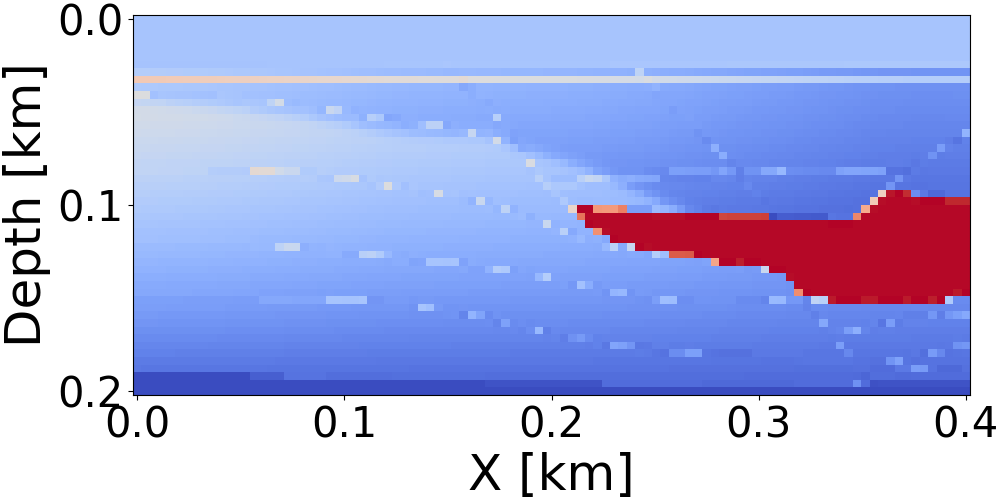
\includegraphics[width=\linewidth]{public/true}
            \vspace{-9mm}
            \caption*{\raisebox{-2mm}{Ground truth}}
            \vspace{1mm}
        \end{minipage} &
        \hspace{-5mm}
        \begin{minipage}[b]{\linewidth}
            \centering
            
\includegraphics[width=\linewidth]{public/initial}
            \vspace{-9mm}
            \caption*{\raisebox{-2mm}{Initial model}}
            \vspace{1mm}
        \end{minipage} &
        \hspace{-8mm}
        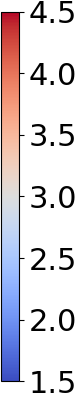
\includegraphics[height=25mm]{public/color-bar}
    \end{tabular}
    \vspace{-3mm}
    \caption{subsurface properties for experiments}
    \label{fig:experiment-data}
\end{figure}

\begin{figure}[t]
    \centering
    \begin{tabular}{m{0mm} m{40mm} m{40mm} m{20mm}}
        % dummy
        \begin{minipage}[b]{\linewidth}\end{minipage} &

        \begin{minipage}[b]{\linewidth}
            \centering
            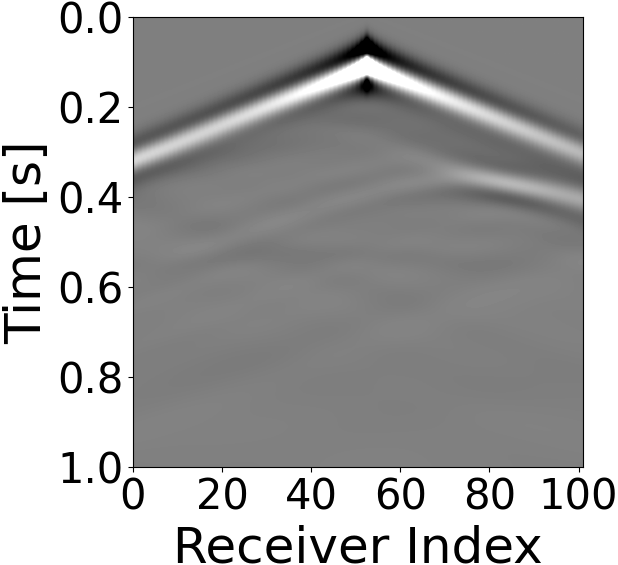
\includegraphics[width=\linewidth]{public/seismic_data}
%            \vspace{-7mm}
            \caption*{\raisebox{-2mm}{Seismic Data}}
%            \vspace{1mm}
        \end{minipage} &
        \begin{minipage}[b]{\linewidth}
            \centering
%            \vspace{1mm}
            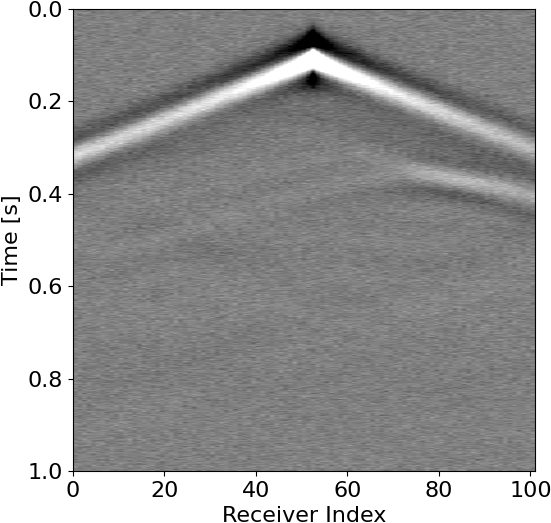
\includegraphics[width=\linewidth]{public/seismic_data_noisy}
%            \vspace{-7mm}
            \caption*{\raisebox{-2mm}{Noisy Seismic Data}}
%            \vspace{1mm}
        \end{minipage} &
        \hspace{-3mm}
        \multirow[t]{3}{*}{\raisebox{-11mm}{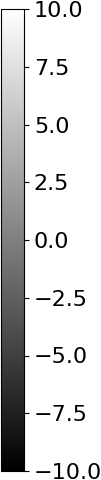
\includegraphics[height=35mm]{public/seismic-data-color-bar}}} \\
    \end{tabular}
%    \vspace{-4mm}
    \caption{The sinthesized seismic data corresponding to a single source waveform.}
%    \vspace{-5mm}
    \label{fig:observed-seismic-data}
\end{figure}


\begin{figure*}[htbp]
    \centering
    \begin{tabular}{m{43mm} m{43mm} m{43mm} m{43mm} m{10mm}}
        \hspace{-3mm}
        \begin{minipage}[b]{\linewidth}
            \centering
            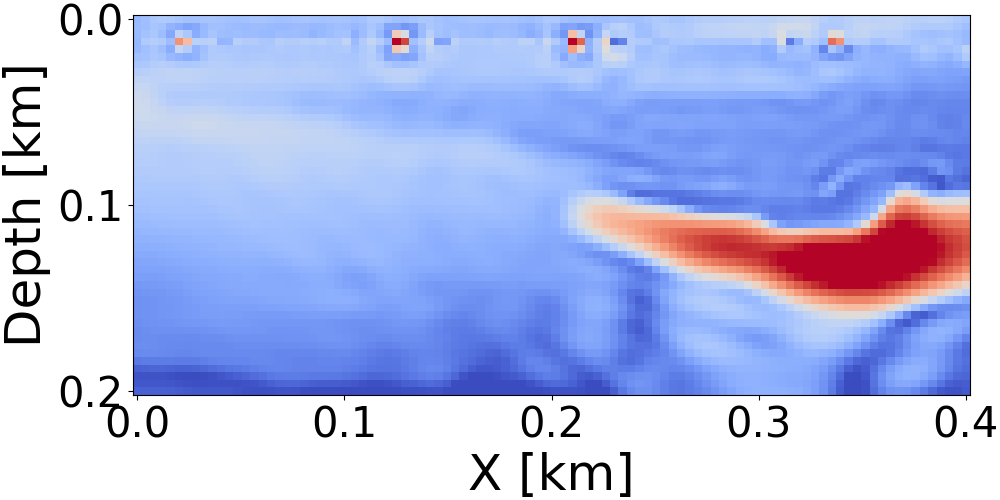
\includegraphics[width=\linewidth]{public/gradient}
%            \vspace{-6mm}
            \caption*{(a) Standard FWI}
%            \vspace{1mm}
        \end{minipage} &
        \hspace{-8mm}
        \begin{minipage}[b]{\linewidth}
            \centering
            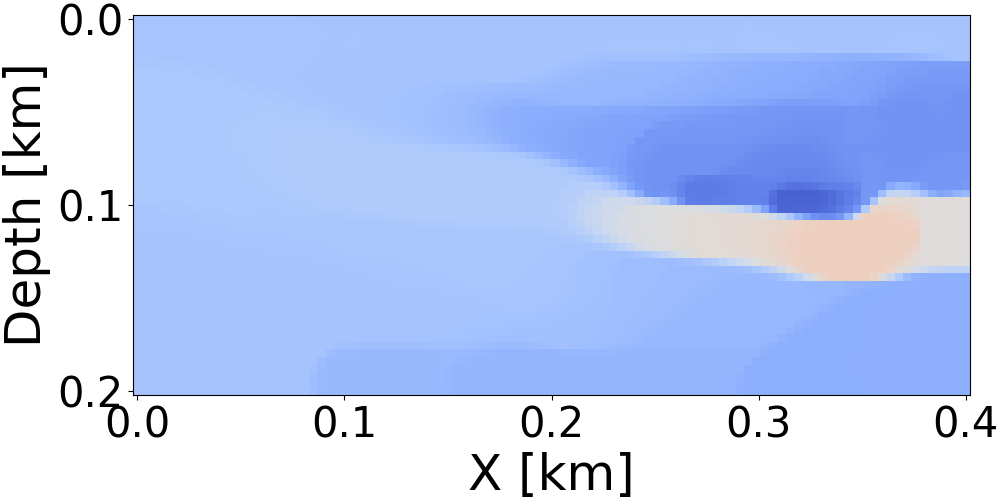
\includegraphics[width=\linewidth]{public/alpha_150}
%            \vspace{-6mm}
            \caption*{(b) Proposed, $\alpha$ = 150}
%            \vspace{1mm}
        \end{minipage} &
        \hspace{-13mm}
        \begin{minipage}[b]{\linewidth}
            \centering
            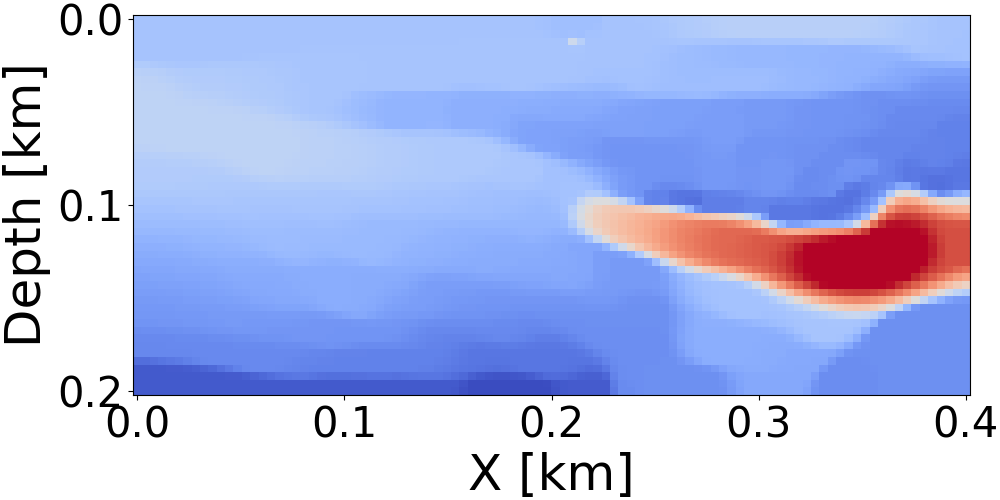
\includegraphics[width=\linewidth]{public/alpha_350}
%            \vspace{-6mm}
            \caption*{(c) Proposed, $\alpha$ = 350}
%            \vspace{1mm}
        \end{minipage} &
        \hspace{-18mm}
        \begin{minipage}[b]{\linewidth}
            \centering
            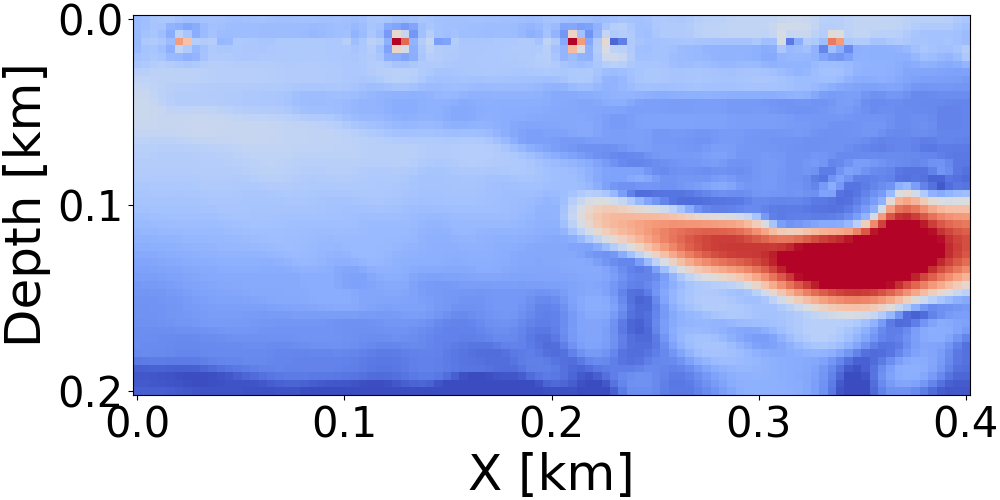
\includegraphics[width=\linewidth]{public/alpha_550}
%            \vspace{-6mm}
            \caption*{(d) Proposed, $\alpha$ = 550}
%            \vspace{1mm}
        \end{minipage} &
%        \hspace{-18mm}
%        \multirow[t]{3}{*}{\raisebox{-5mm}{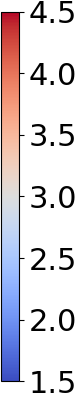
\includegraphics[height=20mm]{public/color-bar}}} \\
    \end{tabular}
%    \vspace{-3mm}
    \captionsetup{margin=1cm}
    \caption{
        Velocity models [km/s] and their corresponding reconstructions. (c) is the best reconstruction result. \\
        (b) is over-smoothed with a stronger TV constraint, and (d) similar results to (a) with a weaker one.
    }
%    \vspace{-4mm}
    \vspace{1mm}
    \label{fig:velocity-models-pure}
\end{figure*}

\begin{figure*}[htbp]
    \centering
    \begin{tabular}{m{43mm} m{43mm} m{43mm} m{43mm} m{10mm}}
        \hspace{-3mm}
        \begin{minipage}[b]{\linewidth}
            \centering
            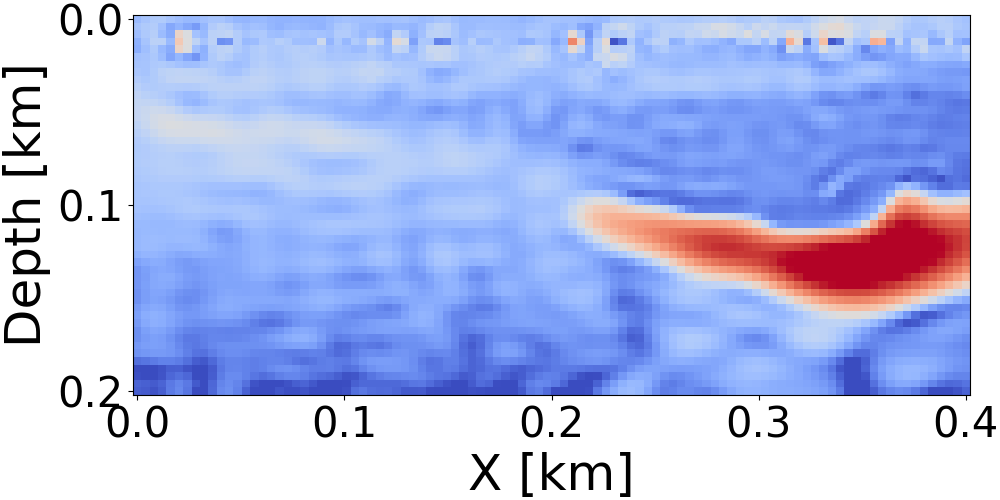
\includegraphics[width=\linewidth]{public/gradient_noisy}
            \vspace{-6mm}
            \caption*{(e) Standard FWI}
            \vspace{1mm}
        \end{minipage} &
        \hspace{-8mm}
        \begin{minipage}[b]{\linewidth}
            \centering
            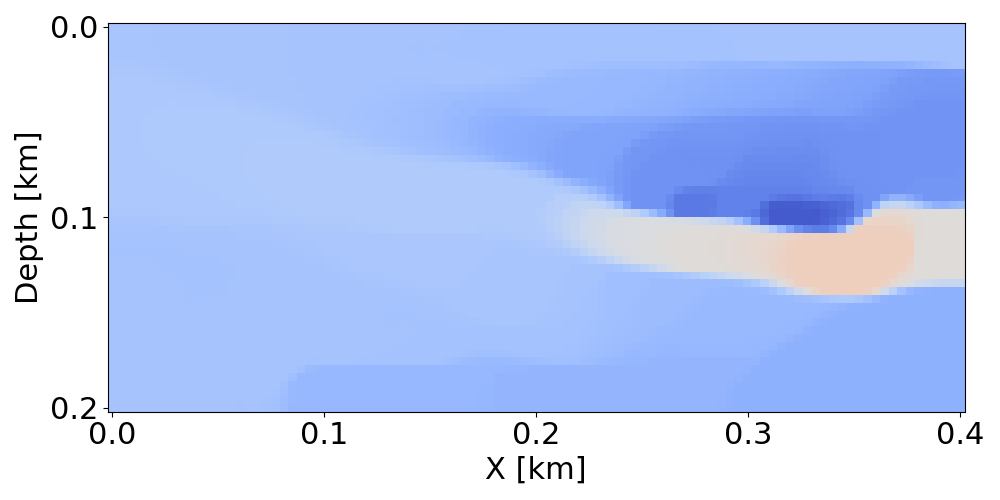
\includegraphics[width=\linewidth]{public/alpha_150_noisy}
            \vspace{-6mm}
            \caption*{(f) Proposed, $\alpha$ = 150}
            \vspace{1mm}
        \end{minipage} &
        \hspace{-13mm}
        \begin{minipage}[b]{\linewidth}
            \centering
            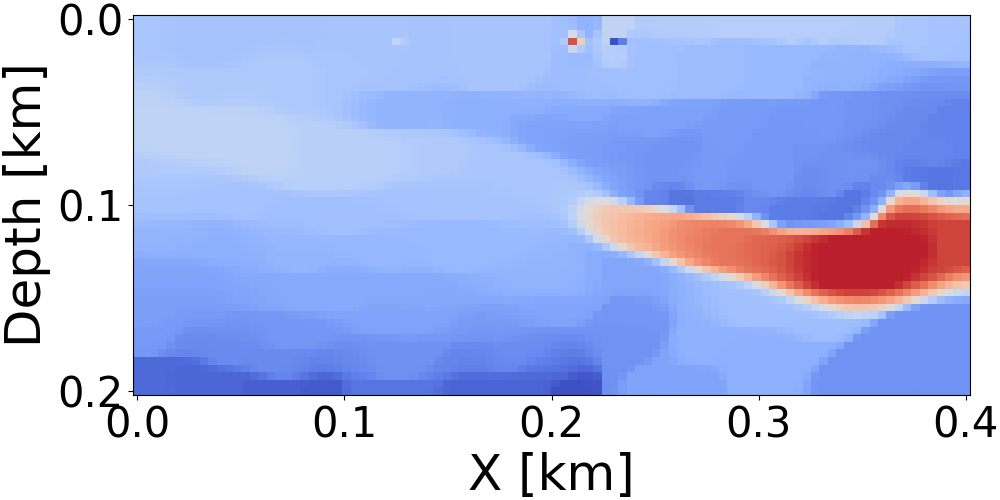
\includegraphics[width=\linewidth]{public/alpha_350_noisy}
            \vspace{-6mm}
            \caption*{(g) Proposed, $\alpha$ = 350}
            \vspace{1mm}
        \end{minipage} &
        \hspace{-18mm}
        \begin{minipage}[b]{\linewidth}
            \centering
            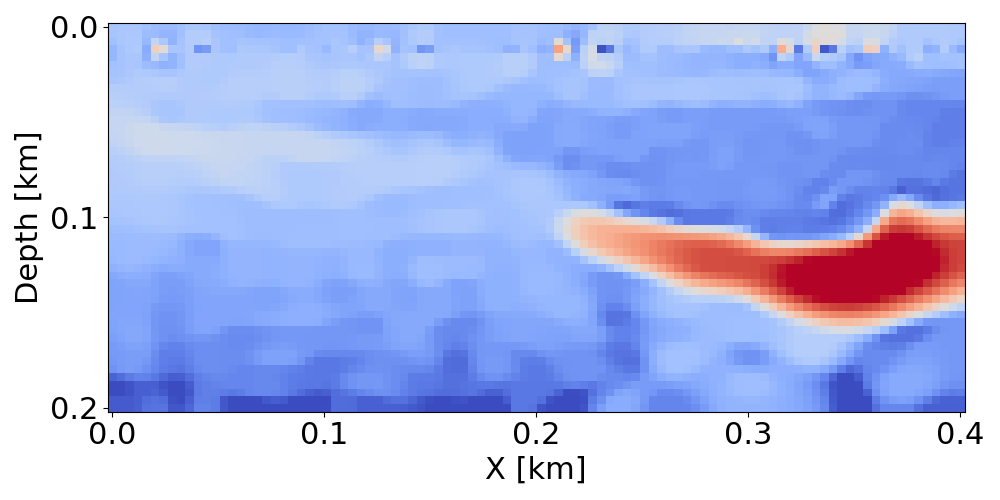
\includegraphics[width=\linewidth]{public/alpha_550_noisy}
            \vspace{-6mm}
            \caption*{(h) Proposed, $\alpha$ = 550}
            \vspace{1mm}
        \end{minipage} &
        \hspace{-21.5mm}
        \multirow[t]{3}{*}{\raisebox{-2.7mm}{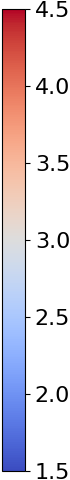
\includegraphics[height=40mm]{public/color-bar-min}}} \\
    \end{tabular}
    \vspace{-3mm}
    \captionsetup{margin=1cm}
    \caption{
        Velocity models [km/s] and their corresponding reconstructions (with the noisy data). Similar to Fig.~\ref{fig:velocity-models-pure}, (g) is the best result, and (f)/(h) are the results with stronger/weaker TV constraint.
    }
    \vspace{-2mm}
    \label{fig:velocity-models-noisy}
\end{figure*}

\begin{figure*}[htbp]
    \centering
    \hspace{-3mm}
%    \begin{minipage}{58mm}
%        \centering
%        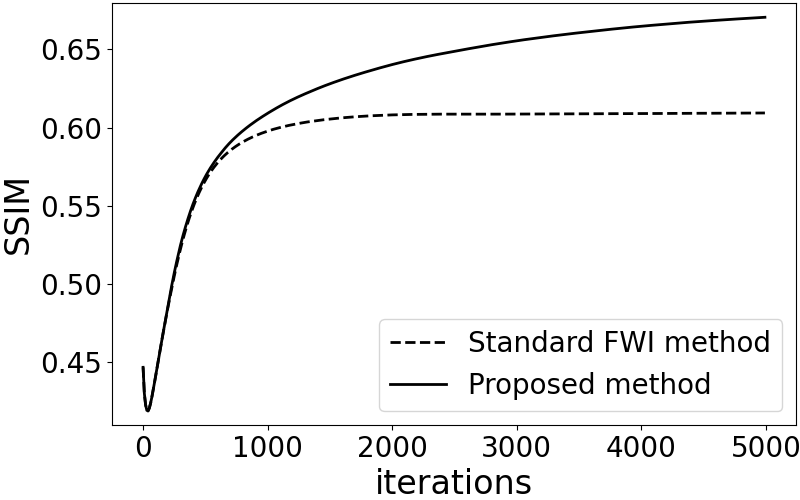
\includegraphics[width=\linewidth]{public/iters-ssim}
%%        \vspace{-6mm}
%        \caption{SSIM against iters.}
%        \label{fig:iters-ssim}
%        \vspace{-2mm}
%    \end{minipage}
%    \hspace{-1mm}
    \begin{minipage}{58mm}
        \centering
        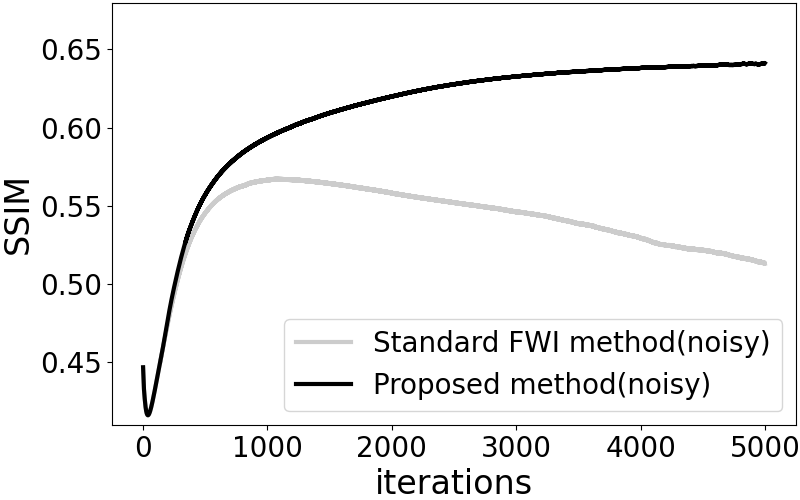
\includegraphics[width=\linewidth]{public/iters-ssim-noisy}
%        \vspace{-6mm}
        \caption{SSIM against iters. (noisy)}
        \label{fig:iters-ssim-noisy}
        \vspace{-3mm}
    \end{minipage}
    \hspace{-1mm}
    \begin{minipage}{58mm}
        \centering
        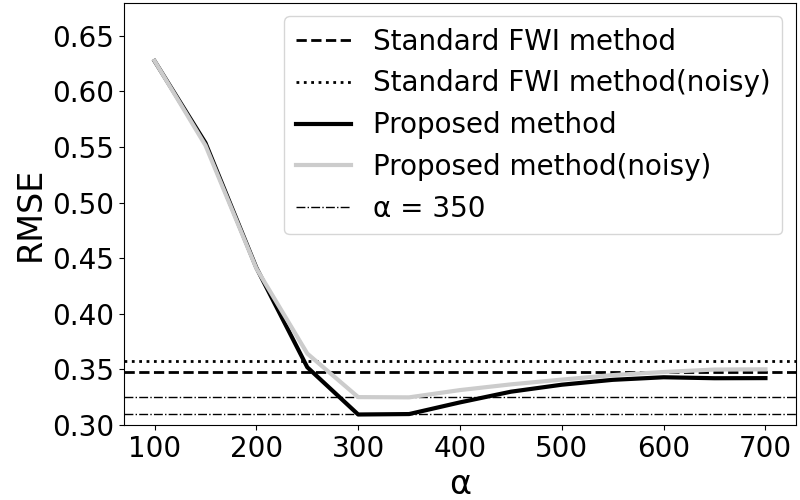
\includegraphics[width=\linewidth]{public/alpha-rmse-edited}
%        \vspace{-6mm}
        \caption{RMSE against $\alpha$.}
        \label{fig:alpha-rmse}
        \vspace{-3mm}
    \end{minipage}
    \hspace{-2mm}
    \begin{minipage}{58mm}
        \centering
        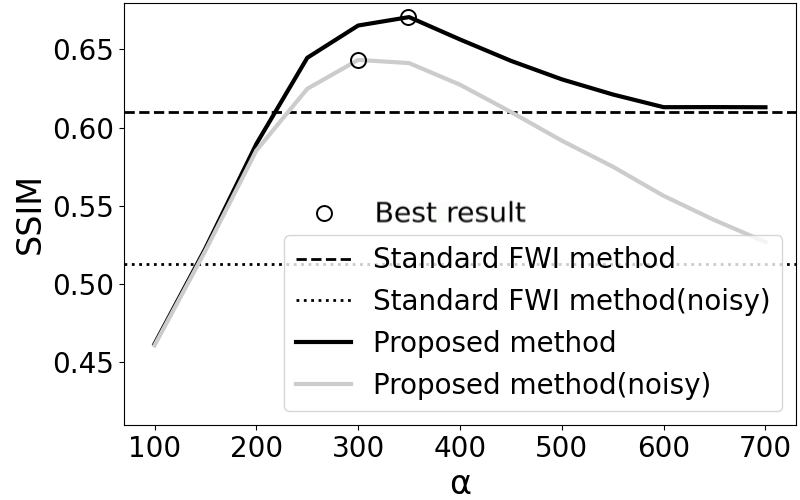
\includegraphics[width=\linewidth]{public/alpha-ssim-all-edited}
%        \vspace{-6mm}
        \caption{SSIM against $\alpha$.}
        \label{fig:alpha-ssim}
        \vspace{-3mm}
    \end{minipage}
\end{figure*}





\subsection{Results and Discussion} \label{subsec:results-and-discussion}
First, we present the experimental results without noise in the observed seismic data.
Fig.~\ref{fig:velocity-models-pure} shows the reconstructed velocity models using the standard FWI method and the proposed methods with $\alpha$ = 150, 350, and 550.
The best parameter is $\alpha$ = 350, where $\alpha$ = 150 represents a stronger TV constraint and $\alpha$ = 550 represents a weaker one.
The standard FWI method generates wave-like artifacts throughout.
In contrast, our proposed method with the best parameter, which is $\alpha$ = 350, achieves the accurate velocity model reconstruction without these artifacts.
As shown in Fig.~\ref{fig:alpha-rmse} and Fig.~\ref{fig:alpha-ssim}, the proposed method archive accurate reconstruction performance, as evidenced by quantitative evaluations using the Root Mean Squared Error (RMSE) and the Structural Similarity Index Measure (SSIM).
The case of $\alpha$ = 150, 550 will be discussed later.

%For quantitative evaluation, Fig.~\ref{fig:iters-ssim} shows the Structural Similarity Index Measure (SSIM) against the number of iterations for our proposed method and the standard FWI method.
%The proposed method consistently achieves higher SSIM values than the standard FWI method at every iteration, indicating enhanced reconstruction accuracy.

Second, we present the experimental results with the noisy observed seismic data.
Fig.~\ref{fig:velocity-models-noisy} shows the reconstructed velocity models using the standard FWI method and the proposed methods with $\alpha$ = 150, 350 and 550.
In the FWI problem with the noisy observed seismic data, the standard FWI method generates stronger wave-like artifacts throughout.
In contrast, our proposed method with $\alpha$ = 350 as the appropriate parameter still achieves accurate velocity model reconstruction without these artifacts and achieves almost the same level of performance as in the noiseless case.
This demonstrates the robustness of the reconstruction accuracy to noise in the observed seismic data.

Fig.~\ref{fig:iters-ssim-noisy} shows the SSIM against the number of iterations for our proposed method and the standard FWI method.
The standard FWI method with the noisy observed seismic data degrades the SSIM after a certain number of iterations.
On the other hand, the proposed method maintains a consistently high value without degrading the SSIM even after a large number of iterations.
This shows that the proposed method effectively reduces the risk of overfitting to noisy data, providing stable and accurate performance even as the number of iterations increases.

For a more detailed analysis of the TV constraint parameter $\alpha$, we plot the RMSE and SSIM of our proposed method against the parameter $\alpha$ and the standard FWI method in Fig.~\ref{fig:alpha-rmse} and Fig.~\ref{fig:alpha-ssim}.
When around $\alpha$ = 350, the proposed method achieves the best RMSE and SSIM.
When $\alpha$ is smaller, the TV constraint becomes stronger, the RMSE and SSIM worsens, and over-smoothing occurs, as in Fig.~\ref{fig:velocity-models-pure} and Fig.~\ref{fig:velocity-models-noisy} for $\alpha$ = 150.
On the other hand, when $\alpha$ is larger, the TV constraint becomes weaker and the result is similar to the standard FWI method, as in Fig.~\ref{fig:velocity-models-pure} and Fig.~\ref{fig:velocity-models-noisy} for $\alpha$ = 550.
However, thanks to the box constraint, the proposed method still outperforms the standard FWI method.
This demonstrates that the parameter $\alpha$ has a clear and predictable effect on the reconstructed velocity model, which can be easily adjusted to achieve accurate results.

